\begin{figure}[t]
\centering
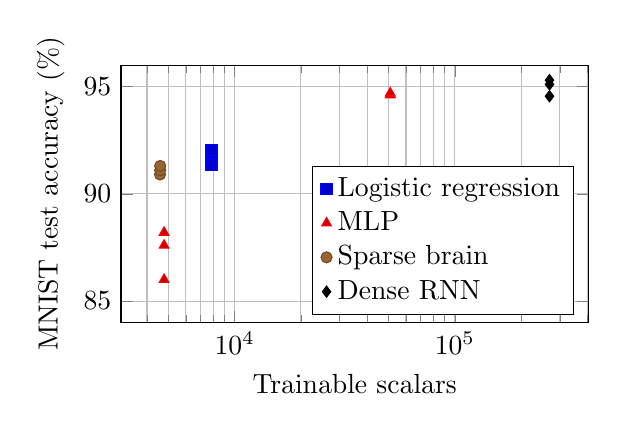
\begin{tikzpicture}
\begin{axis}[width=0.62\textwidth, height=0.4\textwidth, xlabel={Trainable scalars}, ylabel={MNIST test accuracy (\%)}, xmode=log, grid=both, legend pos=south east, legend cell align=left, ymin=84, ymax=96]
\addplot+[mark=square*, only marks] coordinates {(7850,91.35) (7850,91.90) (7850,92.05)};
\addplot+[mark=triangle*, only marks] coordinates {(4780,86.00) (4780,87.60) (4780,88.20) (50890,94.60) (50890,94.65) (50890,94.70)};
\addplot+[mark=*, only marks] coordinates {(4580,90.90) (4588,91.10) (4589,91.30)};
\addplot+[mark=diamond*, only marks] coordinates {(269066,94.55) (269066,95.10) (269066,95.30)};
\legend{Logistic regression, MLP, Sparse brain, Dense RNN}
\end{axis}
\end{tikzpicture}
\caption{Parameter efficiency on MNIST (10k training digits, 3 seeds). The sparse brain sits at 4.6k trainable scalars between the parameter-matched MLP and the wide baselines; it does not beat a linear classifier.}
\label{fig:params}
\end{figure}
